\subsection{ADC Control} \label{subsec:ADC_CONTROL} 

The ADC control block is the controlling hardware for the two external LTC2311\cite{ADC_LTC2311} ADCs that are being used to sample the DUT voltage and current waveforms. The module should, when it sees a rising edge from another HDL block, start a sampling process through the ADCs, clock the data out of the ADCs, latch the data and set a data\_ready flag for the IV saver block to read the sampled data as shown on figure \refq{fig:7_2_8_ADCControlProcess}. This section will only concern itself with the timing of the ADC and the communication between the ADC and FPGA.

\begin{figure}[H]
    \centering
    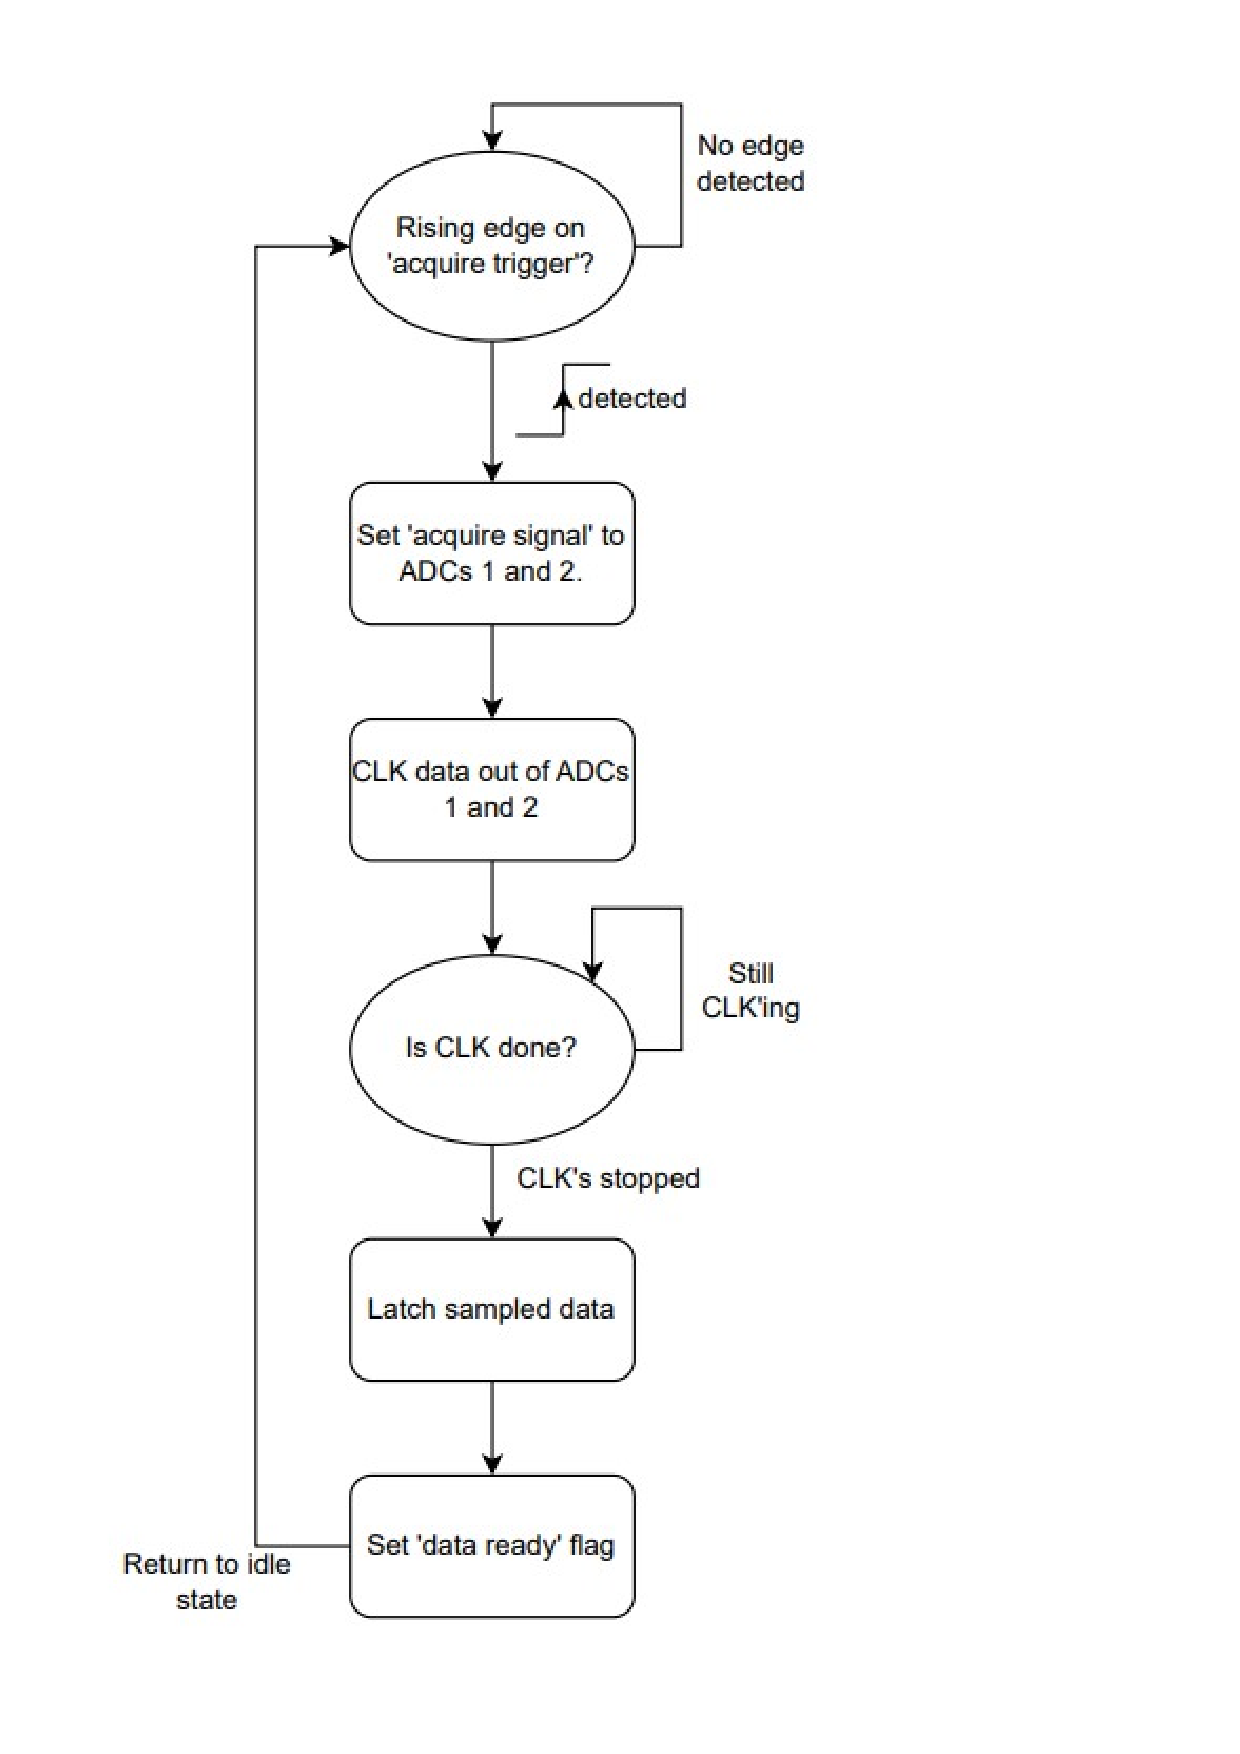
\includegraphics[clip, trim=0 0 0 0, width=0.6\textwidth]{Sections/7_SystemDesign/Figures/7_2_8_ADCControlOverallSignals_cropped.pdf}
    \caption{A process flow showing the overall function of the ADC control block. The block is 'triggered' on a rising edge of an input signal. The block will set an 'acquire' signal to the ADCs, which will start a sample and hold and AD-conversion process. The block will then clock out the sampled data, latch it, and let the next HDL block know that there is sample data ready for processing.}
    \label{fig:7_2_8_ADCControlProcess}
\end{figure}

In order to make the process flow in figure \refq{fig:7_2_8_ADCControlProcess} work the ADC control block must fulfill the timing requirements of the LTC2311 ADC. The timings can be seen on figure \refq{fig:7_2_8_LTC2311_TIMING} where some significant periods have been marked in red on the timing diagram. These will be explained in detail. 

\begin{figure}[H]
    \centering
    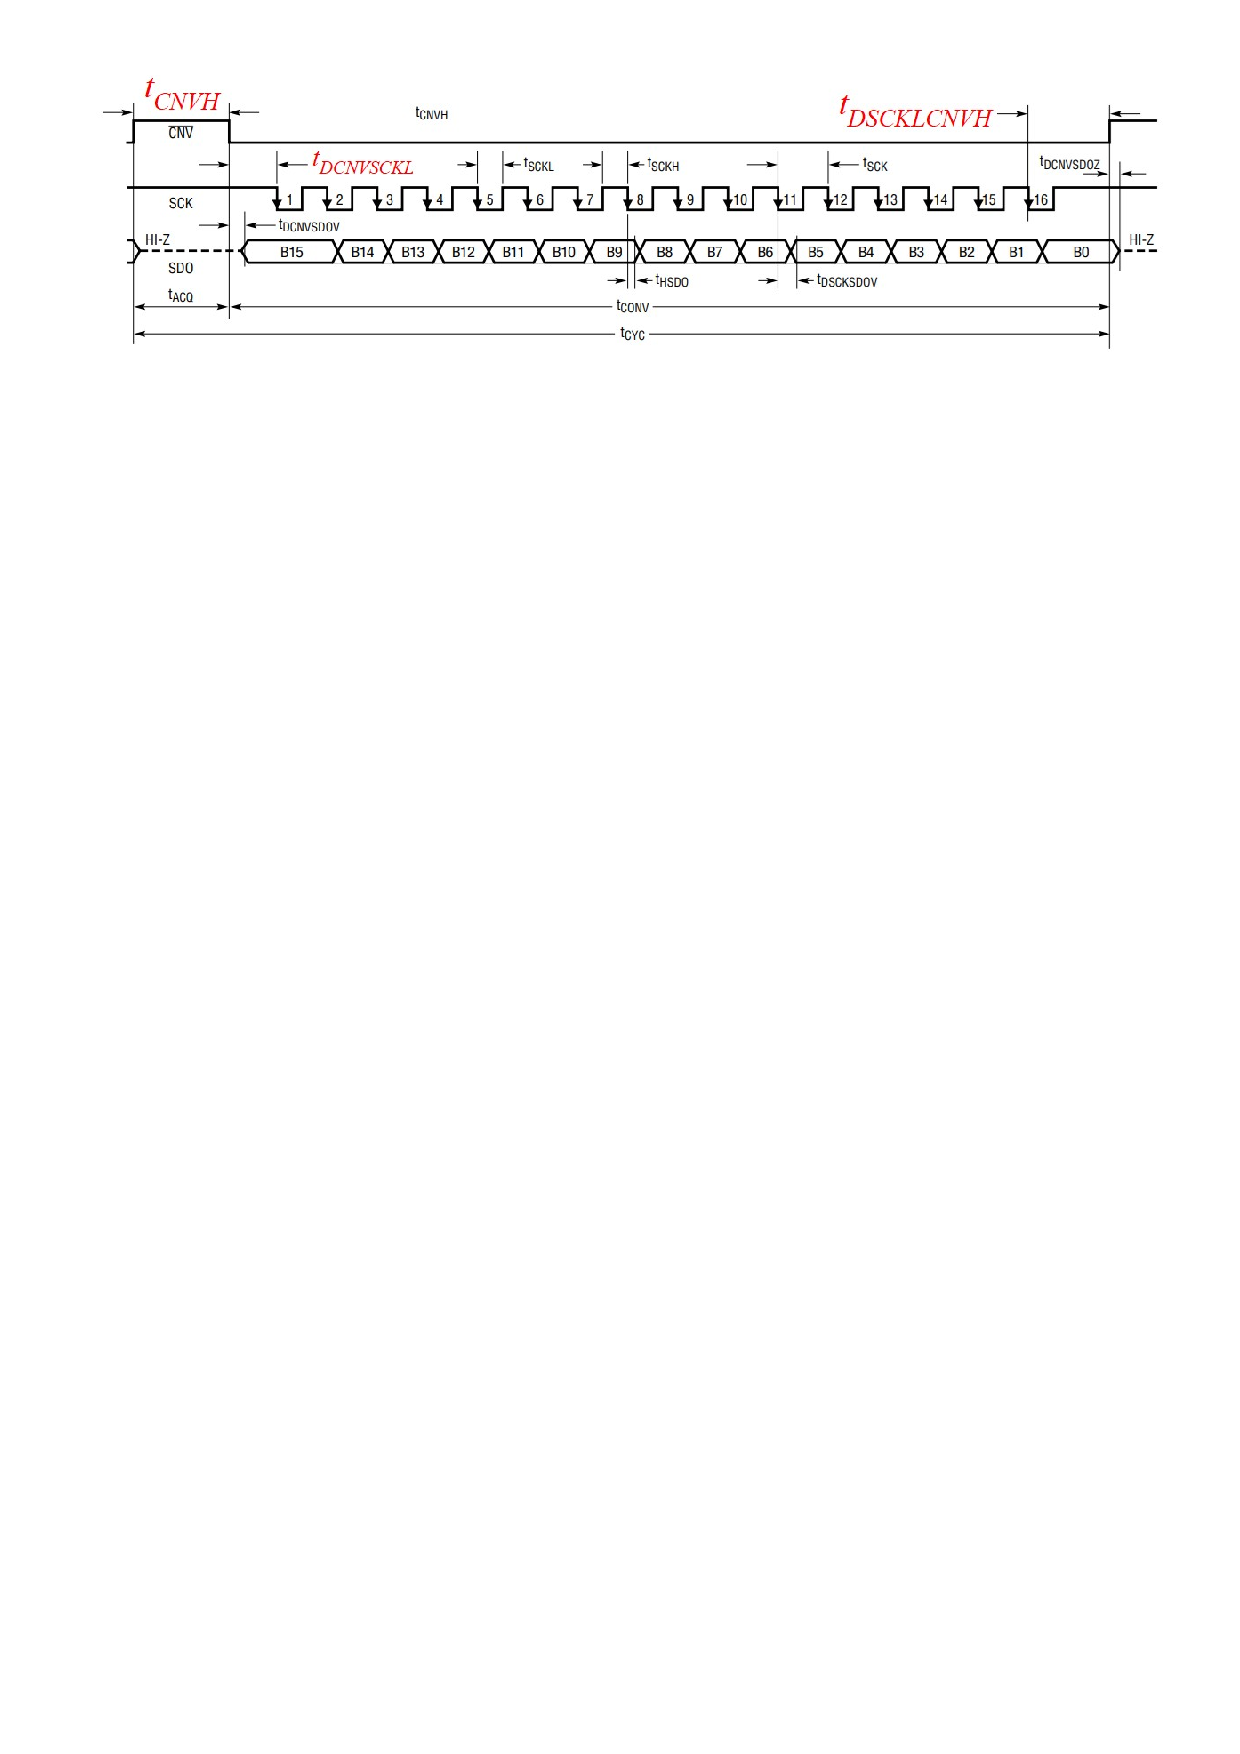
\includegraphics[clip, trim=0 675 0 0, width=1\textwidth]{Sections/7_SystemDesign/Figures/7_2_8_LTC2311_TIMING.pdf}
    \caption{A timing diagram of the communication between the LTC2311 ADC and an SPI master.}
    \label{fig:7_2_8_LTC2311_TIMING}
\end{figure}

The ADC starts an acquisition, i.e. samples the input, when the CNV signal transitions from '0' to '1' and digitizes the value during the $t_{CNVH}$ time. FIgure \refq{fig:7_2_8_LTC2311_TIMING} also lists this time as the acquisition time, $t_{ACQ}$. This time is important and the datasheet suggests $t_{CNVH} = 30 ns$ for a $5M sps$ sample rate. The ADC control block will be designed for a sample rate of $1 Msps$, even though the actual sample rate is expected to be much lower at this point. The main CLK in the sample control module is a \SIQ{200}{\mega\hertz} CLK with a period of $t_{clk} = 5 ns$, so any multiple of this clock signal will be convenient for generating the CNV pulse. The CNV pulse width will be $t_{CNVH} = 35 ns$ for the project.

The DCN pulse is when data is clocked out on the bus..

The DSC pulse is the time from the last data is clocked to the bus and when a new acquisition can start....